\documentclass[12pt,a4paper]{exam}

% --------------------
% Packages
% --------------------
\usepackage[utf8]{inputenc}
\usepackage[T1]{fontenc}
\usepackage[french]{babel}
\usepackage{amsmath,amssymb}
\usepackage{geometry}
\usepackage{pgfplots}
\pgfplotsset{compat=1.18}
\geometry{margin=2cm}

% --------------------
% En-tête / pied (exam)
% --------------------
\header{\textbf{NOM Prénom : }}{}{1ère STMG}
\footer{}{\thepage}{}

% --------------------
\begin{document}

\begin{center}
    \Large\textbf{Interrogation\\Probabilités conditionnelles}
\end{center}

\vspace{0.3cm}

\noindent
\textbf{Durée :} 30min \hfill
\textbf{Calculatrice :} \underline{NON} autorisée

\vspace{0.5cm}

% ======================================================
\noindent
\textbf{Exercice 1 : Des agriculteurs (\ \ \ \  / 6 points )}

\vspace{10pt}
Un agriculteur embauche des salariés et des saisonniers pour les travaux de récolte ou 
des travaux d'entretien, selon le tableau suivant.

\vspace{-5pt}
\begin{center}
    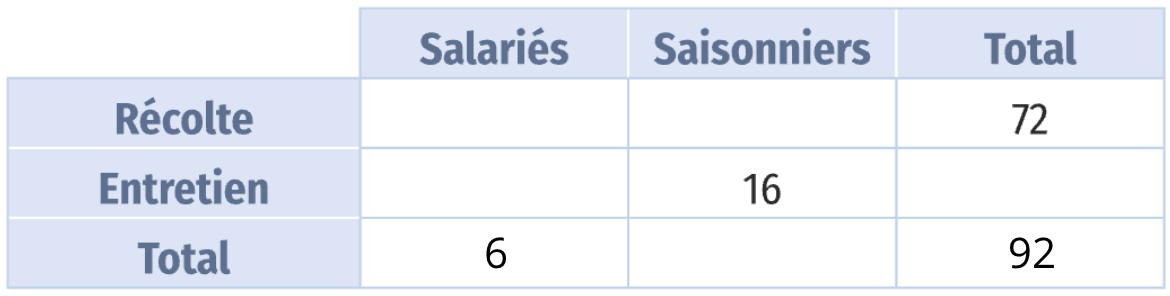
\includegraphics[width=0.7\textwidth]{fig3.png}
\end{center}


\begin{questions}

\question[1] Complétez le tableau sachant qu'un salarié sur trois travaille en récolte.

\question[1] On choisit une personne au hasard travaillant pour cet agriculteur. Quelle 
est la probabilité qu'elle fasses des travaux d'entretien ?

\question[2] On choisit un saisonnier au hasard. Quelle est la probabilité qu'il travaille à 
la récolte ?

\question[2] On choisit un récolteur au hasard. Quelle est la probabilité qu'il soit salarié ?
\end{questions}

\vspace{1cm}

% ========================================================
%             Exercice 2
% ========================================================
\noindent
\textbf{Exercice 2 : Un spectacle ( \ \ \ / 4 points )}

\vspace{10pt}
Un spectacle propose 1630 places à la vente, en guichet ou sur Internet.
Les places ont toutes été vendues. 1181 ont été vendues sur Internet, et parmi elles, 
476 ont été vendues le jour même. 884 ont été vendues la semaine précédente et parmi elles,
179 ont été vendues au guichet.

\vspace{5pt}
On note S l'évènement : « Le spectateur a acheté son billet la semaine précédente »

On note J l'évènement : « Le spectateur a acheté son billet le jour même »

On note G l'évènement : « Le spectateur a acheté son billet au guichet »

On note I l'évènement : « Le spectateur a acheté son billet sur Internet »


\begin{questions}

\question[2] Sachant que le spectateur a acheté sa place sur Internet, quelle est la probabilité 
qu'il ait acheté sont billet le joour même ?

\question[2] Calculer $P_{S}(G)$.

\end{questions}

\vspace{0.5cm}

\begin{center}
    \textit{Fin du devoir}
\end{center}

\end{document}
